% Created 2022-08-29 lun 23:42
% Intended LaTeX compiler: pdflatex
\documentclass[12pt]{article}
\usepackage[utf8]{inputenc}
\usepackage[T1]{fontenc}
\usepackage{graphicx}
\usepackage{grffile}
\usepackage{longtable}
\usepackage{wrapfig}
\usepackage{rotating}
\usepackage[normalem]{ulem}
\usepackage{amsmath}
\usepackage{textcomp}
\usepackage{amssymb}
\usepackage{capt-of}
\usepackage{hyperref}
\usepackage[spanish]{babel}
\usepackage{graphicx,geometry}
\geometry{ a4paper, left=1in, right=1in, top=1in, bottom=1in }
\renewcommand\familydefault{\sfdefault}
\usepackage{sectsty}
\sectionfont{\normalfont\large }
\usepackage{tabularx}
\usepackage{listings}
\lstdefinestyle{mystyle}{
numbers=left,
showspaces=false,
frame=leftline,
showspaces=false,
showstringspaces=false,
showtabs=false,
numberstyle=\tiny,
}
\lstset{
style=mystyle,
literate={á}{{\'a}}1
{é}{{\'e}}1
{í}{{\'{\i}}}1
{ó}{{\'o}}1
{ú}{{\'u}}1
{Á}{{\'A}}1
{É}{{\'E}}1
{Í}{{\'I}}1
{Ó}{{\'O}}1
{Ú}{{\'U}}1
{ü}{{\"u}}1
{Ü}{{\"U}}1
{ñ}{{\~n}}1
{Ñ}{{\~N}}1
{¿}{{?``}}1
{¡}{{!``}}1
}
\makeatletter
\usepackage{fancyhdr}
\pagestyle{fancy}
\usepackage{mdframed}
\BeforeBeginEnvironment{minted}{\begin{mdframed}}
\AfterEndEnvironment{minted}{\end{mdframed}}
\author{Luis Eduardo Galindo Amaya (1274895)}
\date{2022-08-29}
\title{Exploración de herramientas de modelado}
\hypersetup{
 pdfauthor={Luis Eduardo Galindo Amaya (1274895)},
 pdftitle={Exploración de herramientas de modelado},
 pdfkeywords={},
 pdfsubject={},
 pdfcreator={Emacs 26.3 (Org mode 9.1.9)}, 
 pdflang={Spanish}}
\begin{document}


\newcommand{\docente}{Manuel Castañón-Puga}
\newcommand{\asignatura}{Herramientas de Desarrollo de Software (40017)}
\newcommand{\semestre}{2022-2}

\newcommand{\miportada}[1]{
	\begin{titlepage}
		\vspace*{0.75in}
		\begin{flushleft}
			\sffamily
			\large #1       \\
			\Huge 
            \@title         \\
			\hrulefill
			\vspace{0.25in} \\
			\Large \@author \\
			\vspace*{\fill}
            
\includegraphics[width=\textwidth]{../includes/filler.png} \\
			\vspace*{\fill}
			\large
			\begin{tabular}{|l|l|}
              \hline
			  Asignatura & \asignatura \\
			  Docente    & \docente    \\
			  Fecha      & \@date      \\
              \hline
			\end{tabular}
		\end{flushleft}
	\end{titlepage}
}

\fancyhf{}
\lhead{ \asignatura }
\rhead{ \semestre }
\rfoot{Página \thepage}

\setlength\parindent{0pt}   % eliminar el intentado
\setlength{\parskip}{1.2em}
% \maketitle

\thispagestyle{empty}
\begin{center}
	{\large
		UNIVERSIDAD AUTÓNOMA DE BAJA CALIFORNIA \\
		Facultad de Ciencias Químicas e Ingeniería }
	\vspace{0.25in} \\
	Programa de Ingeniero en Software y Tecnologías Emergentes
\end{center}


\section*{Información De La Materia}
\label{sec:orgc408c03}
\begin{mdframed}
\begin{description}
\item[{Asignatura}] \asignatura .
\item[{Grupo y Periodo}] 341 (2022-2) .
\item[{Docente}] \docente .
\end{description}
\end{mdframed}

\section*{Información De La Actividad}
\label{sec:org9524b47}
\begin{mdframed}
\begin{description}
\item[{Nombre de la actividad}] Exploración de herramientas de modelado.
\item[{Fecha}] 2022-08-29
\item[{Lugar}] Edificio 6E, Salón 204.
\item[{Carácter de la actividad}] Individual.
\item[{Participante(es)}] Luis Eduardo Galindo Amaya (1274895).
\end{description}
\end{mdframed}

\section*{Reporte De Actividades}
\label{sec:org8b3e925}
\subsection*{Explorando Visual Paradigm}
\label{sec:orgbd46073}
\begin{enumerate}
\item Primero cree un proyecto en Visual Paradigm, simplemente se hace clic en '+' uml.
\end{enumerate}
\begin{center}
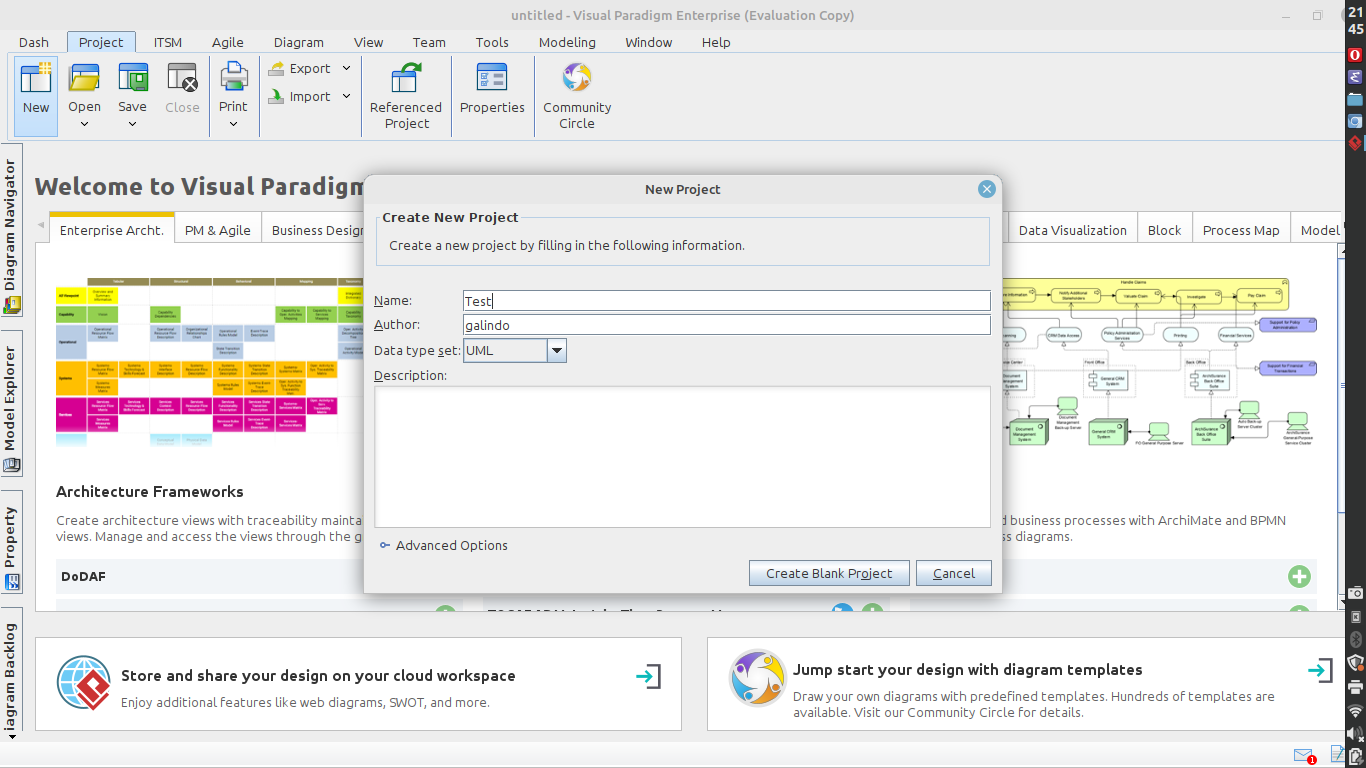
\includegraphics[width=.9\linewidth]{./img/1.png}
\end{center}

\begin{enumerate}
\item después hice un pequeño modelo en UML
\end{enumerate}
\begin{center}
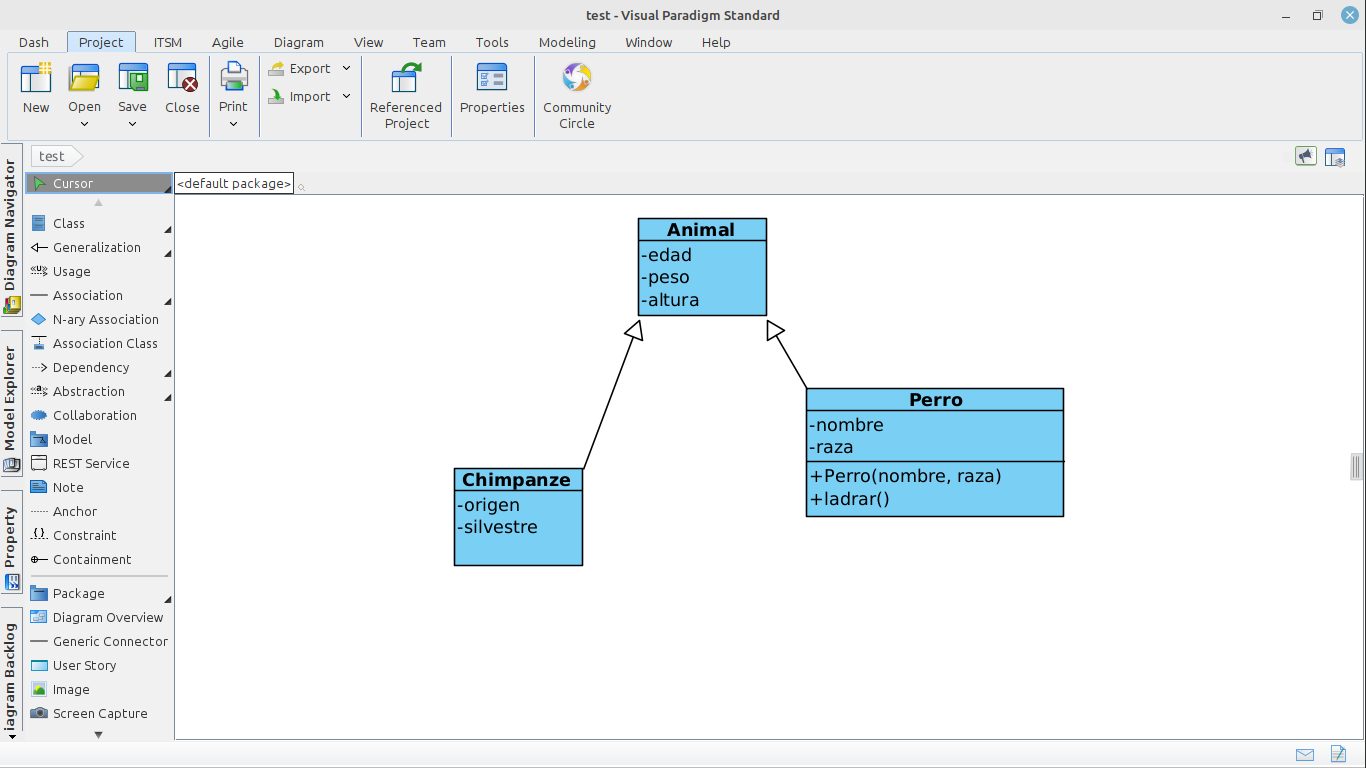
\includegraphics[width=.9\linewidth]{./img/2.png}
\end{center}

\begin{enumerate}
\item exporte el Código del proyecto
\end{enumerate}
\begin{center}
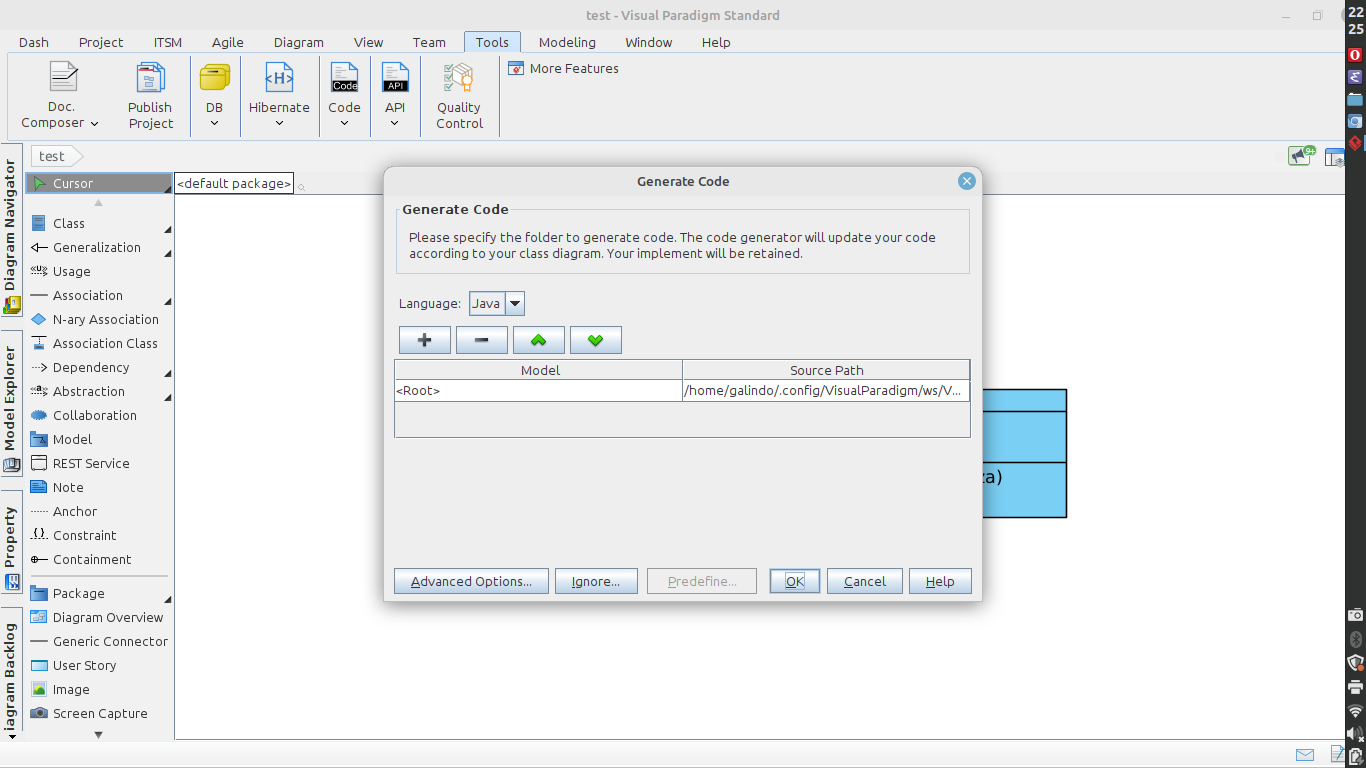
\includegraphics[width=.9\linewidth]{./img/3.png}
\end{center}

\begin{enumerate}
\item y por ultimo lo abrí en pycharm
\end{enumerate}
\begin{center}
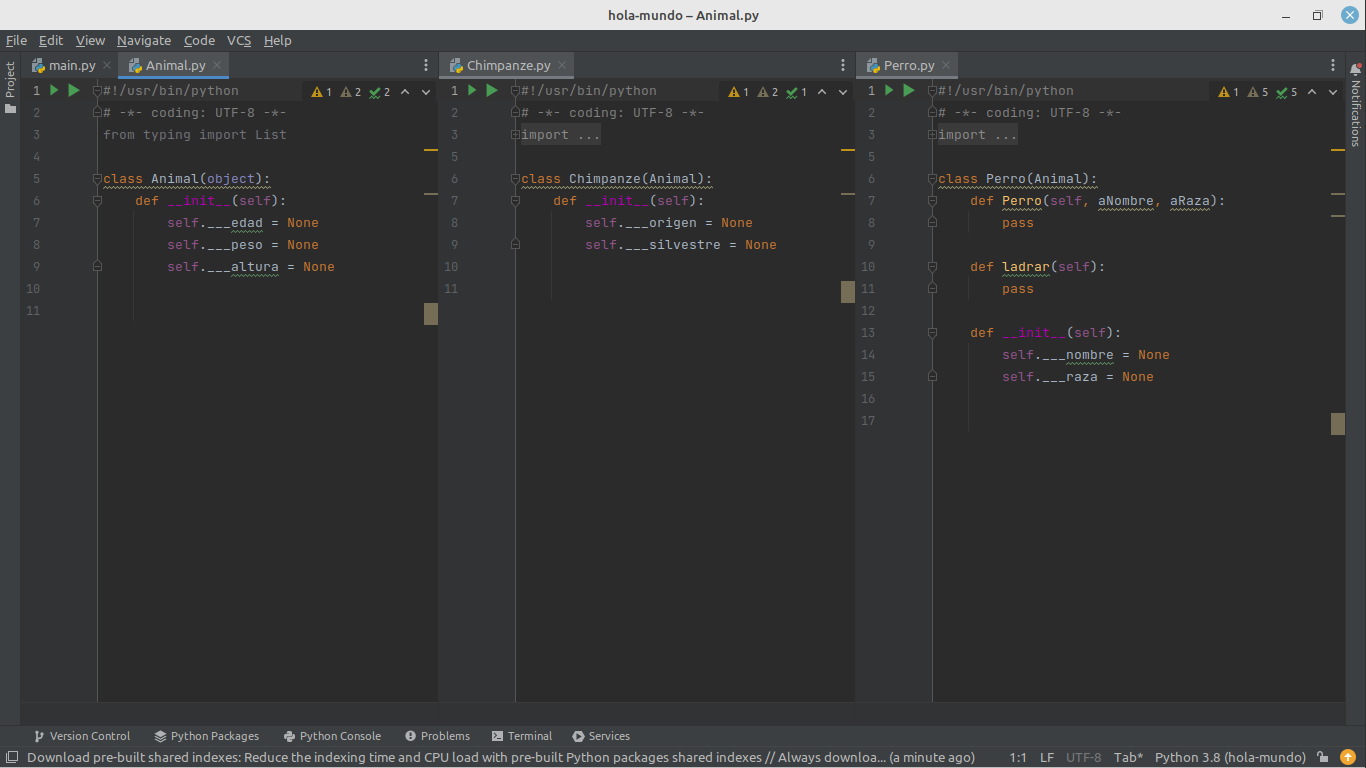
\includegraphics[width=.9\linewidth]{./img/4.png}
\end{center}

\subsection*{Explorando otras herramientas}
\label{sec:orgabaec45}
Mi herramienta por excelencia para hacer diagramas de cualquier tipo es sin duda plantuml, me gusta porque es muy ligera y los diagramas básicamente se pueden hacer con código y se acomodan solos, nada de drag and drop.

Comparando plantuml y Visual Paradigm es fácil ve porque se preferiría visual paradigm, la habilidad de generar código en base al diagrama o viceversa es muy útil, pero Plantuml es mas útil para hacer diagramas para la universidad o pequeños productos.


\section*{Reflexión}
\label{sec:org8e729d1}
\begin{mdframed}
Los diagramas son herramientas muy útiles en cualquier ámbito y las herramientas para generar diagramas son la única alternativa real a hacerlos en papel, hay varios enfoques al mismo problema y debemos buscar cual alternativa es mejor para cada caso individual.
\end{mdframed}

\begin{center}
Doy fe de que toda la información dada es  completa y correcta. \\
\begin{center}

\includegraphics[width=3cm]{../includes/firma.png}
\end{center}
Luis Eduardo Galindo Amaya (1274895)
\end{center}
\end{document}
